
\documentclass{article}

% Recommended (ICML template):
\usepackage{microtype}
\usepackage{graphicx}
\usepackage{subcaption}
\usepackage{booktabs}
\usepackage{hyperref}

% Attempt to make hyperref and algorithmic work together better:
\newcommand{\theHalgorithm}{\arabic{algorithm}}

% ICML style (BLIND SUBMISSION):
\usepackage{icml2026}

% Math + utilities used in your paper:
\usepackage{amsmath}
\usepackage{amssymb}
\usepackage{mathtools}
\usepackage{amsthm}
\usepackage{xspace}
\usepackage{url}
\usepackage{xcolor}
\usepackage{placeins}

% If you use cleveref:
\usepackage[capitalize,noabbrev]{cleveref}

%%%%%%%%%%%%%%%%%%%%%%%%%%%%%%%%
% THEOREMS (keep if needed)
%%%%%%%%%%%%%%%%%%%%%%%%%%%%%%%%
\theoremstyle{plain}
\newtheorem{theorem}{Theorem}[section]
\newtheorem{proposition}[theorem]{Proposition}
\newtheorem{lemma}[theorem]{Lemma}
\newtheorem{corollary}[theorem]{Corollary}
\theoremstyle{definition}
\newtheorem{definition}[theorem]{Definition}
\newtheorem{assumption}[theorem]{Assumption}
\theoremstyle{remark}
\newtheorem{remark}[theorem]{Remark}

% Text shorthands (from your submission)
\newcommand{\ie}{\emph{i.e.,}\xspace}
\newcommand{\etal}{\emph{et al.}\xspace}
\newcommand{\eg}{\emph{e.g.,}\xspace}

% Running title (must be short)
\icmltitlerunning{Babel-formal: Translating Proofs Between Lean and Rocq}

\begin{document}
	
	\twocolumn[
	\icmltitle{Babel-formal: Translation of Proofs Between Lean and Rocq}
	
	% NOTE (ICML double-blind): do not include author info in the initial submission.
	% If you want to keep author blocks for camera-ready, paste them here and switch to:
	% \usepackage[accepted]{icml2026}
	% (The style will then show authors/affiliations.)

	
	\begin{icmlauthorlist}
		\icmlauthor{Théo Stoskopf}{yyy}
		\icmlauthor{Cyril Cohen}{yyy}
		\icmlauthor{Nicolas Tabareau}{xxx}
	\end{icmlauthorlist}
	
	\icmlaffiliation{yyy}{Inria, CNRS, ENS de Lyon,\\
	Université Claude Bernard Lyon 1,\\
	LIP, UMR 5668, Lyon, France}
	\icmlaffiliation{xxx}{Nantes Université, École Centrale Nantes, \\
	CNRS, Inria, \\
	LS2N, UMR 6004, Nantes, France}
	
	\icmlcorrespondingauthor{Théo Stoskopf}{theo.stoskopf@inria.fr}
	\icmlkeywords{formal proof, proof assistants, Lean, Rocq prover, proof translation, large language models, ICML}
	
	\vskip 0.3in
	]
	
	% Required even if empty:
	\printAffiliationsAndNotice{}
	
	\begin{abstract}
		In this work, we investigate using proof terms (the low-level representation of formal proofs) as a pivot language for translating proof scripts between proof assistants and across tactic sets. Unlike direct proof translation, this approach does not require an aligned training corpus; it only needs aligned context at inference time so that both systems elaborate comparable terms. We compare two strategies: (1) direct script-to-script translation with two off-the-shelf LLMs (GPT-5, Qwen2.5-Coder-32B-Instruct), and (2) proof term translation, where an LLM turns a proof term into a proof script in the target language. We build a small benchmark of aligned sources (14 files, 117 lemmas) across Lean and Rocq, and train models to map Lean and Rocq proof terms back to their native proof scripts. Our experiments show that proof term translation works for cross-assistant translation and for translation between tactic sets. It is complementary to using an off-the-shelf LLM for direct proof script translation, scales easily in terms of training data, and handles tactic-set translation better (\eg vanilla Rocq $\to$ SSReflect).
	\end{abstract}
	
	\section{Introduction}
	\begin{figure*}[t]
		\centering
		\begin{minipage}[t]{0.40\textwidth}
			\vspace{0pt}
			\centering
			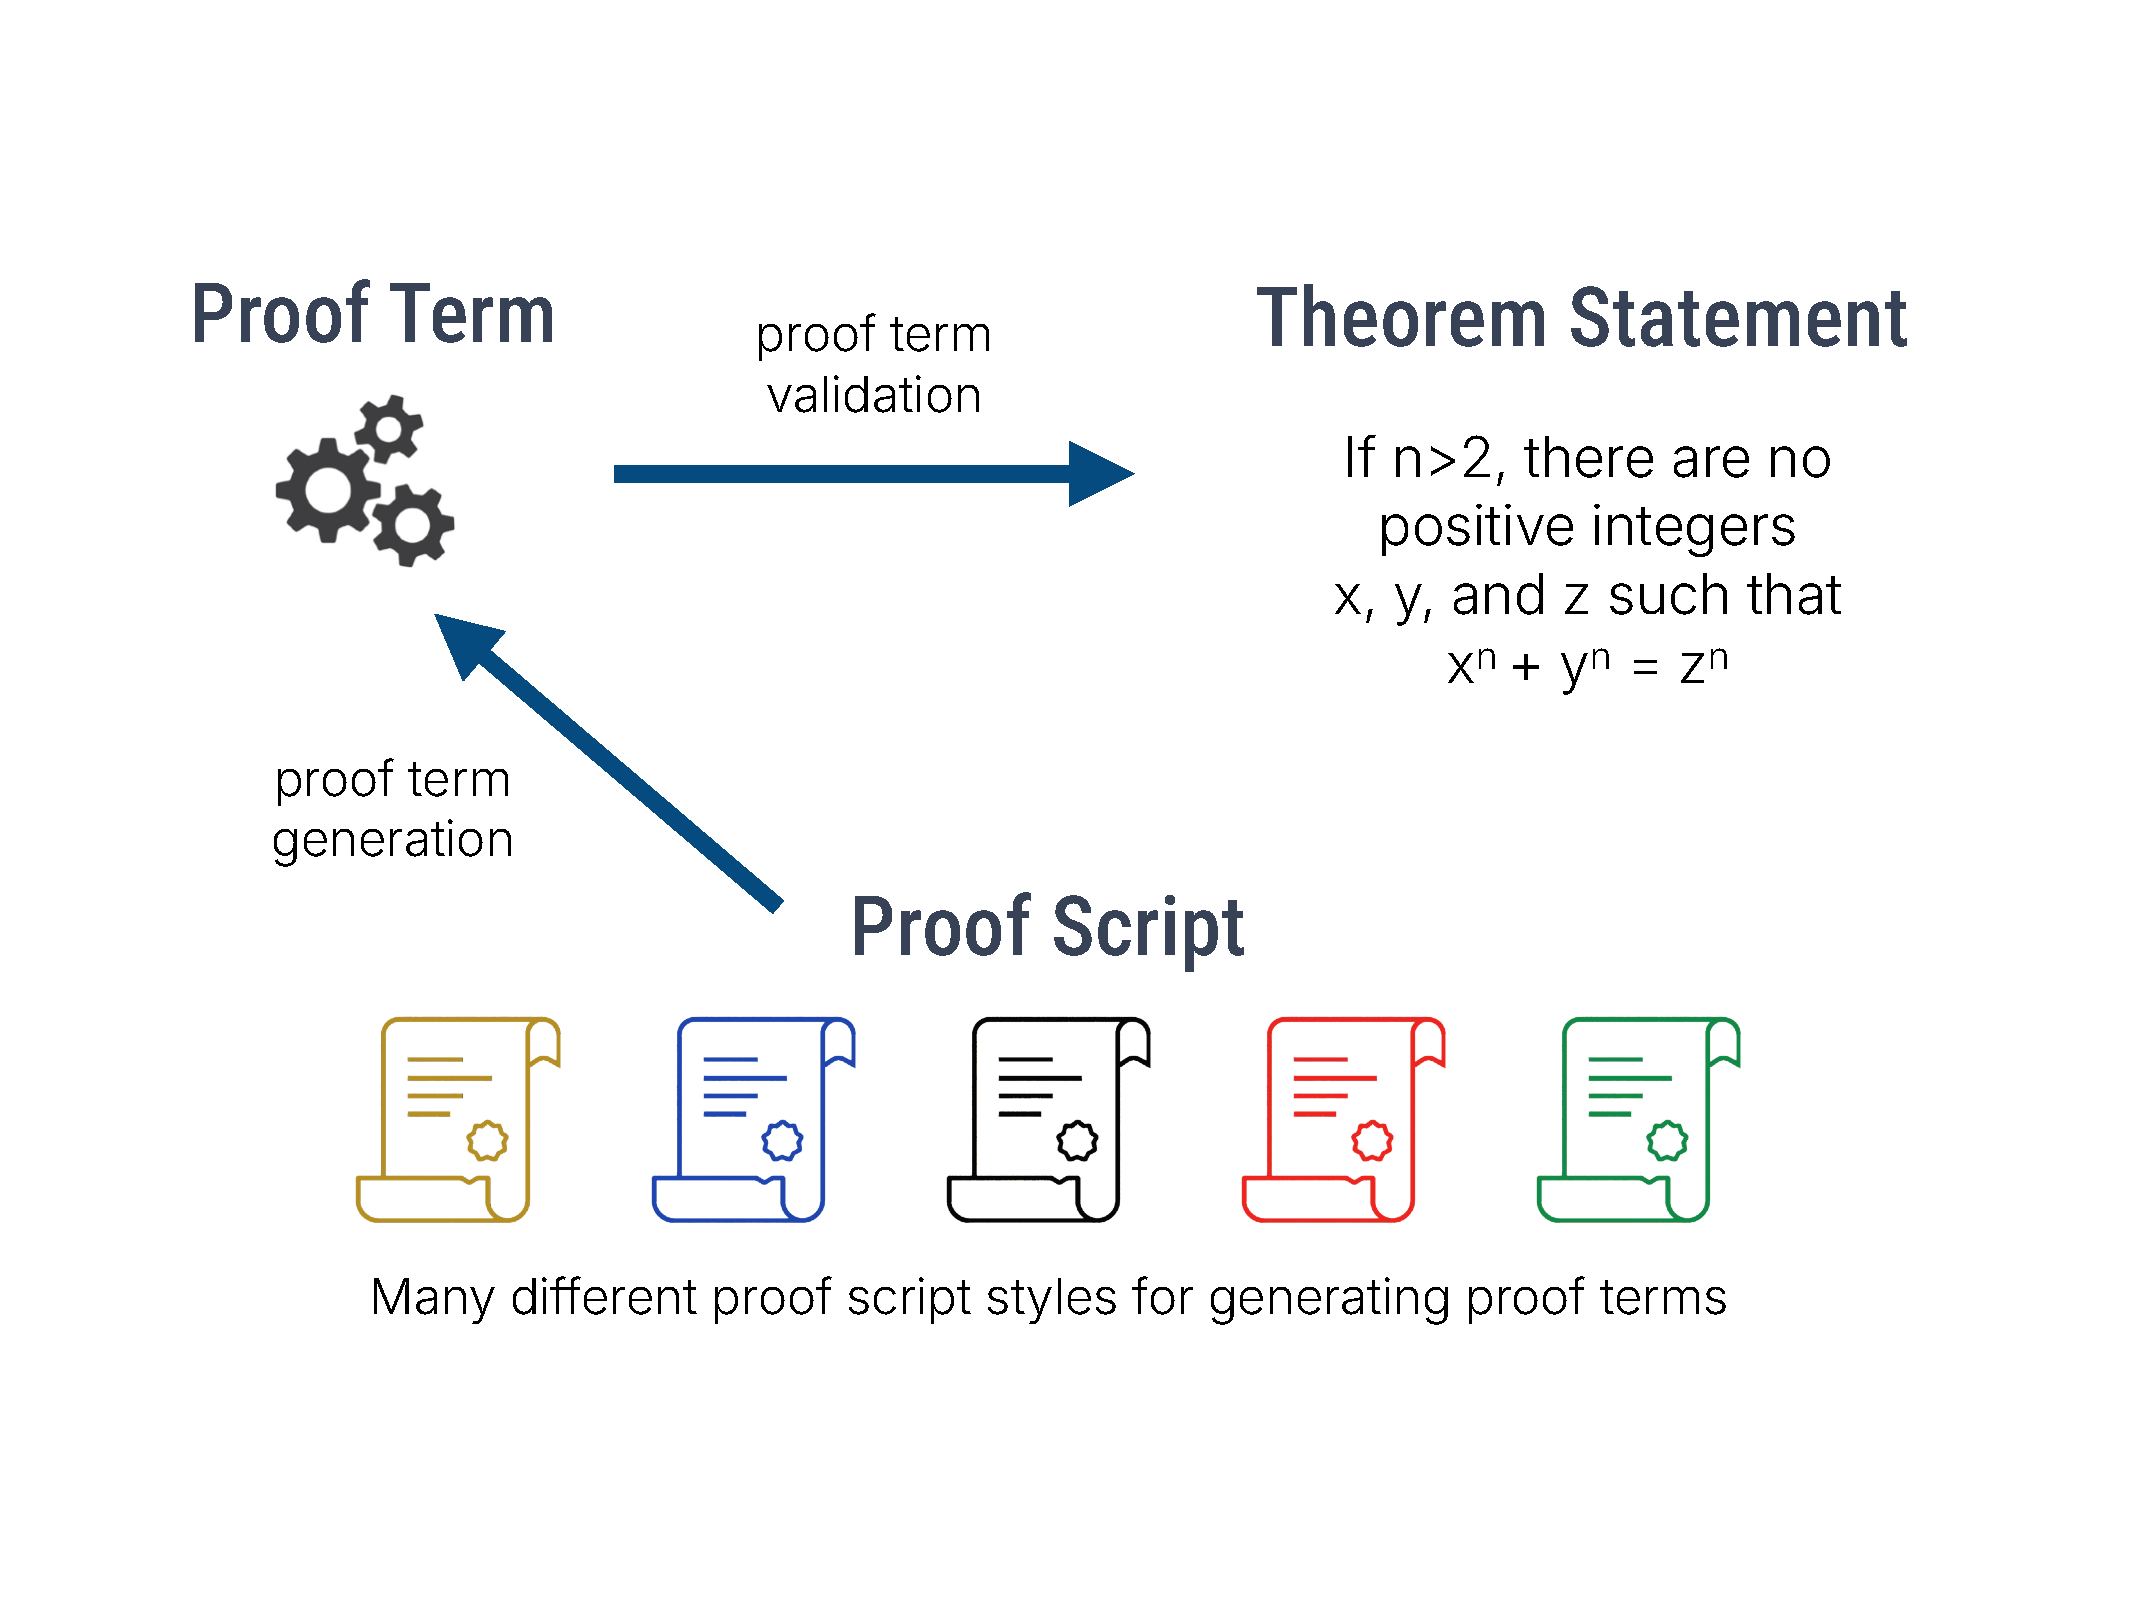
\includegraphics[width=\linewidth]{basic_provers}
		\end{minipage}\hfill
		\begin{minipage}[t]{0.50\textwidth}
			\vspace{0pt}
			\small\raggedright
			Given a formal statement of a theorem, proving it amounts to constructing a proof term, \ie a precise object that the prover can type-check for correctness. However, these proof terms are typically extremely verbose, capturing every low-level detail, and are impractical to write directly by hand.
			
			To address this, users interact with interactive theorem provers through proof scripts, meta-programs designed to generate proof terms. Over time, this layer has evolved, leading to a diverse ecosystem of proof script languages (tactic languages).
		\end{minipage}
		
		\caption{How interactive theorem provers operate.}
		\label{fig:basicprovers}
	\end{figure*}
	Proof assistants such as Rocq and Lean accumulate over time large libraries of formal mathematics (for example, MathComp~\cite{mathcomp} for Rocq and Mathlib~\cite{mathlib} for Lean), yet proofs are not reusable across systems, even in a strictly aligned context. We study two translation settings. The first is \emph{cross-assistant} translation between Lean and Rocq, which is useful to import the many results that exist in one prover but not in the other. The second is \emph{cross-tactic} translation inside Rocq, from the standard Rocq tactic language, called here \textit{vanilla Rocq}, to \textit{SSReflect}~\cite{ssreflect}, which is a compact, structured tactic language widely used with MathComp (see an example in~\cref{app:ssreflect}), and can make existing proofs more robust to changes.
	
	These translation capabilities matter in practice because large verified libraries are not portable: many results exist in one ecosystem but not the other, and re-proving them is costly even when statements are aligned. Beyond reuse, translation also supports migration of existing developments toward more robust proof styles (\eg vanilla Rocq $\to$ SSReflect) without rewriting whole files.
	Finally, our approach is complementary to statement translation. Proof term translation can then fill this gap: once statements are aligned, we can leverage the source proof term to synthesize a proof script that the target assistant can check.
	
	Both Rocq and Lean provide a way to pretty print \emph{proof terms} given by the proof assistant (see~\cref{fig:basicprovers}) in a way that omits details while keeping the structure of a proof. We thus explore using \emph{pretty-printed proof terms} as a pivot language. This removes the need for an aligned training corpus of tactic scripts. At inference time, we only require strictly aligned statements, \ie the same theorem and premises, so that both systems elaborate comparable terms. The approach is related to decompilation in programming languages, where models map assembly to higher-level C programs~\cite{llm4decompile2024}.
	
	We compare two strategies:
	\begin{itemize}
		\item \textbf{Direct script translation.} An LLM is prompted to convert a proof script directly from source tactics to target tactics. We apply this in both settings (Lean~$\leftrightarrow$~Rocq and vanilla Rocq~$\to$~SSReflect), using GPT-5~\cite{gpt52025} as a baseline.
		\item \textbf{Proof term translation.} We first extract the proof term, then train models to predict scripts from proof terms (Lean term to Lean script, Rocq term to Rocq script). At inference, we extract the term for the source proof and use the model to produce a script in the target assistant or tactic set (see~\cref{fig:inference}). For an example of Lean~$\to$~Rocq inference see~\cref{app:leanrocq}, and~\cref{app:ssreflect} for vanilla Rocq~$\to$~SSReflect.
	\end{itemize}
	
	To support this comparison, we build a benchmark of 14 files with 117 lemmas that are strictly aligned between Lean and Rocq. 
	
	Our main contributions are:
	\begin{itemize}
		\item \textbf{Two term-to-script models}, trained to reconstruct proof scripts from pretty-printed proof terms. \textit{Babel-translate} is a single term-to-script model trained on both (Lean term$\to$Lean script) and (Rocq term$\to$Rocq script); at inference, we perform cross-assistant translation by prompting it to emit tactics in the target language while providing the source term. \textit{Babel-ssreflect} translates Rocq proof terms directly into SSReflect scripts, enabling cross-tactic translation from vanilla Rocq proofs to SSReflect within Rocq.
		\item \textbf{A small aligned benchmark} (14 files, 117 lemmas) between Lean and Rocq, with an evaluation of cross-assistant and cross-tactic translation.
                \end{itemize}
                
	\section{Related Work}

        The problem of translating proofs, definitions, and theories
        between interactive theorem provers has been long standing
        goal, driven by the desire to reuse formal developments,
        compare foundations, and transfer results across systems with
        distinct logical cores and computational behaviors.

        A classical approach relies on logical frameworks as common
        targets for translation. Systems such as LF and its
        extensions~\cite{harper1993framework} provide a
        minimal meta-language in which a wide range of deductive
        systems can be encoded. 
        %
        Another influential line of research is based on foundational
        proof certificates~\cite{chihani:hal-00906485}, which aim to
        validate proofs originating from different systems using a
        small, trusted kernel. Rather than translating proofs
        wholesale, this approach extracts evidence that can be
        independently checked. While attractive from a trust
        perspective, FPCs are not primarily designed for proof reuse
        or round-trip translation between interactive systems.

        A significant body of recent work uses Dedukti~\cite{Dedukti}, an
        implementation of the $\lambda\Pi$-calculus modulo rewriting,
        as an intermediate language for interoperability. Dedukti’s
        support for user-defined rewrite rules makes it possible to
        faithfully represent the definitional equalities of diverse
        proof systems within a uniform framework. This approach has
        enabled the translation of proofs and libraries from HOL-Light
        to Coq via Dedukti~\cite{Blanqui2024TranslatingHOLLight}, as
        well as more general translations of definitions and theorems
        between proof
        systems~\cite{FrédéricBlanqui2024Libraries}. Dedukti has also
        been used to translate proofs across different type-theoretic
        fragments, including translations from impredicative to
        predicative systems~\cite{FelicissimoBlanquiBarnawal2023}.

        There also exists a tool for performing a direct, low-level
        translation of terms from Lean to
        Rocq~\cite{leantypechecker}, exploiting the close similarity
        between the core type theories of the two systems.
        
        However, in all those works, translations typically operate at
        a low level, losing the structure and automation present
        in the source proof assistants---and thus do not provide a
        proof script that can be maintained and extended.
        

        
	\section{Methodology}
	
	\begin{figure*}[t]
		\centering
		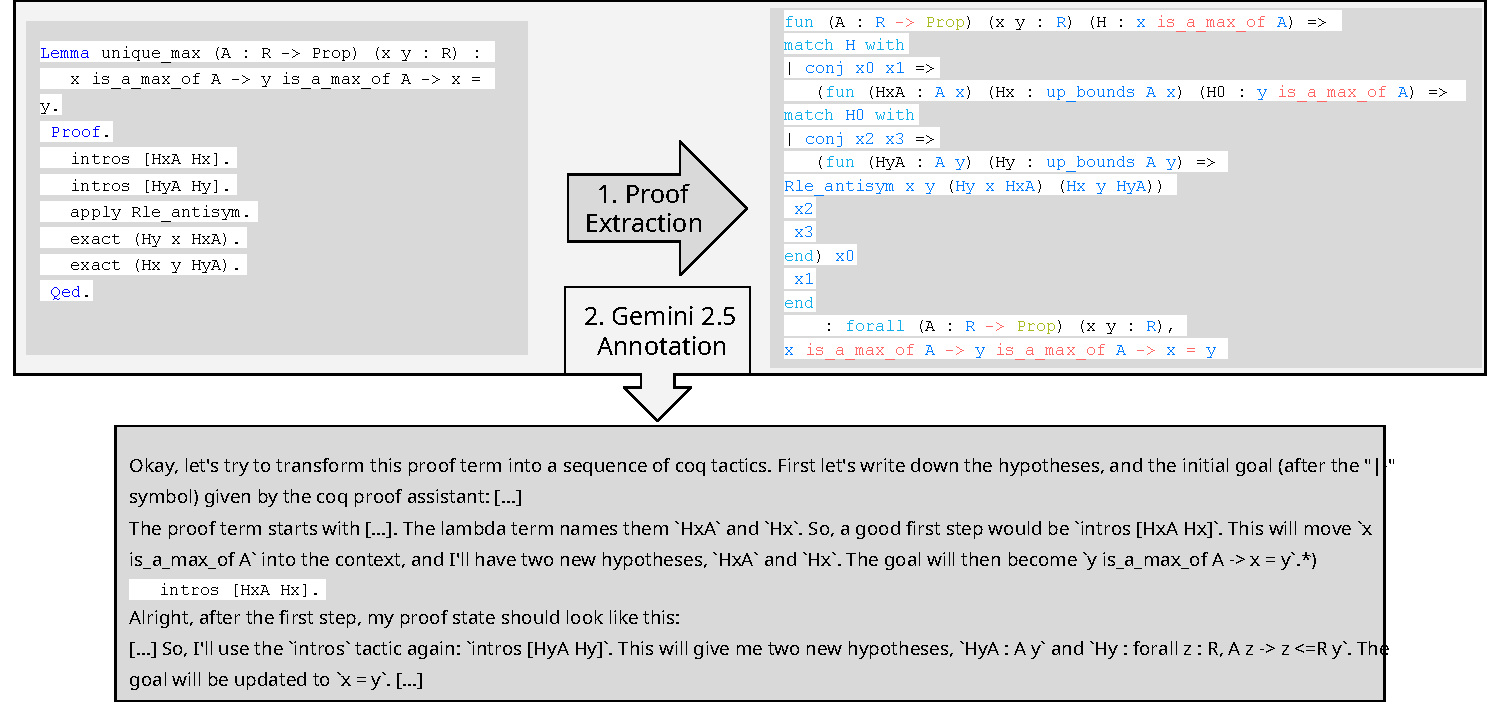
\includegraphics[width=\linewidth]{data_extraction}	
		\caption{Last two steps of dataset collection.}
		\label{fig:data_extraction}
	\end{figure*}
	
	\begin{figure*}[!h]
		\centering
		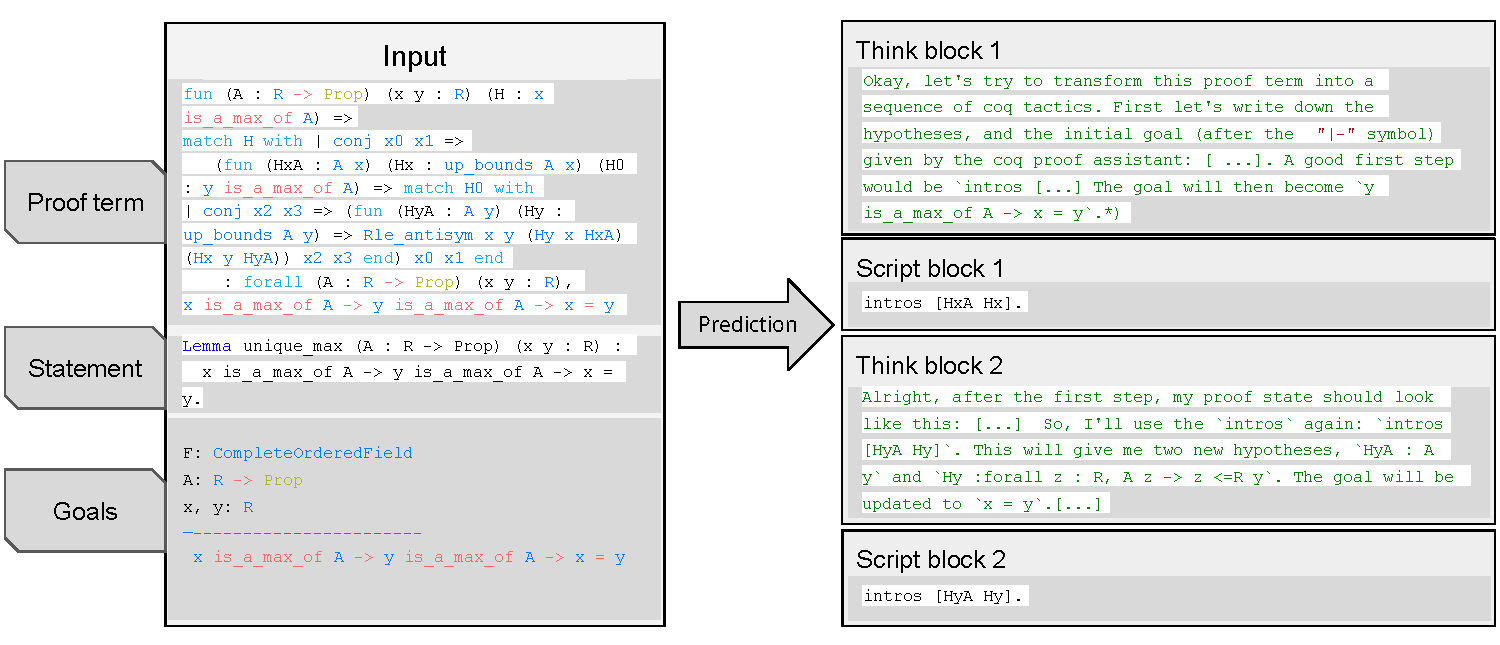
\includegraphics[width=\linewidth]{training}	
		\caption{Training.}
		\label{fig:training}
	\end{figure*}
	
	\begin{figure*}[!h]
		\centering
		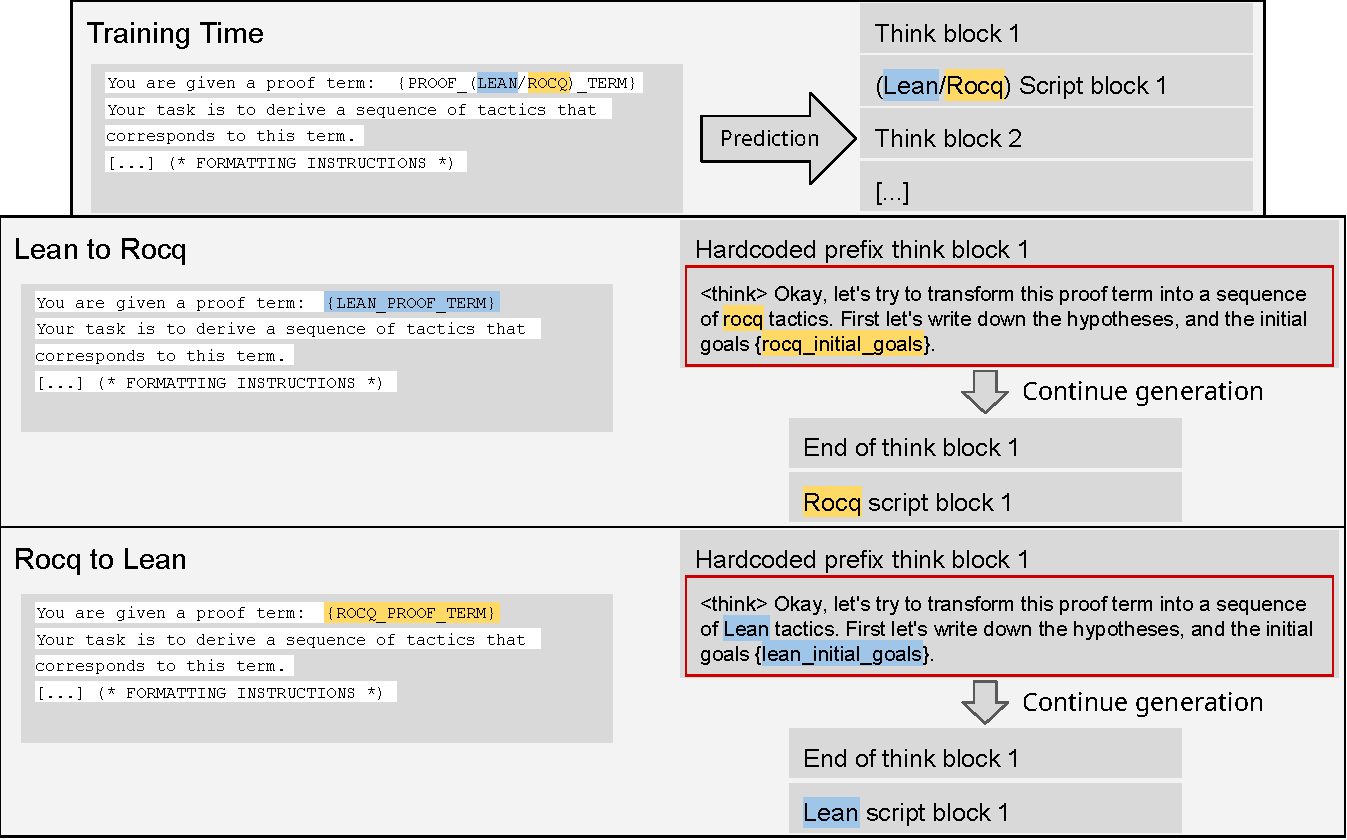
\includegraphics[width=\linewidth]{inference}	
		\caption{Inference strategy.}
		\label{fig:inference}
	\end{figure*}
	
	We describe how we build the training data, the inference pipeline, and benchmarks. To build the training data we follow four steps~\cite{s12025}: (1) select a diverse subset of proofs, (2) extract proof terms in Rocq and Lean, (3) generate synthetic backward reasoning traces inferring proof script from proof term, and (4) train models that predict both  tactic script and reasoning trace from a proof term(~\cref{fig:data_extraction}). Full prompt templates and training details are in~\cref{app:promptbabel,app:training}.
	
	\paragraph{Proof Subset Selection.}
	Following S1~\cite{s12025}, we create in each case a training set of 1000 entries. For translation between Lean and Rocq, we select a subset of 500 diverse proofs in C-CoRN~\cite{corn} and 500 diverse proofs in Mathlib. For translation from vanilla Rocq to SSReflect, we select a subset of 1000 entries in MathComp. In both cases, we filter by length, then choose a diverse subset (statements and proofs) using \texttt{BM25}~\cite{bma}.
	\label{proofextract}
	
	\paragraph{Proof Term Extraction.}
	For Rocq, we use \texttt{coqpyt}~\cite{coqpyt2024} to extract, for each proof, its proof term together with the premises and notation declarations. For Lean~4, we use \texttt{leanclient}~\cite{leanclient2025} to extract the proof term and the context.
	
	\paragraph{Backward Reasoning Trace Generation.}
	Given each proof term and the corresponding target script, we generate backward reasoning traces with Gemini~2.5~Pro~\cite{gemini2024}. Backward reasoning trace generation refers here to prompting the LLM with the proof term and the target proof script, and asking it to generate a reasoning process that works backwards from the script. The resulting training dataset follows the structure described in~\cref{fig:data_extraction}.
	
	\paragraph{Benchmarks.}
	\label{benchmarks}
	We evaluate on two benchmarks:
	
	\emph{Cross-assistant (Lean \texorpdfstring{$\leftrightarrow$}{<->} Rocq).}
	We created 14 files with the same statements in Rocq and Lean, for a total of 117 aligned lemmas. Preparing files took about 20 hours of manual effort in total. Each lemma is proved natively in both systems, so the proof scripts differ but are type-correct in aligned contexts.
	We call two statements \emph{aligned} if they express the same mathematical content under a fixed mapping of definitions and notations, and if they type-check in aligned local contexts (\ie same premises and imports up to that mapping).
	In practice, we created paired Rocq/Lean files by porting statements lemma-by-lemma, keeping the dependency surface small and explicit, and checking that both files compile.
	From these, we extracted comparable proof terms in both systems. An example of such a source file is in~\cref{app:benchmark}.
	
	\emph{Cross-tactic (vanilla Rocq \texorpdfstring{$\to$}{->} SSReflect).}
	We collect 500 Rocq proofs from the C-CoRN library~\cite{corn}, which is developed in vanilla Rocq (in contrast to MathComp, which is built on SSReflect). We use these proofs to assess translation from vanilla Rocq tactics to SSReflect. To ensure diversity, we pick subsets maximizing document distance (via BM25). An example entry is in~\cref{app:ssreflect}.
	
	\paragraph{Limitations.}
	Our aligned benchmark is small and manually constructed. We view it as a controlled testbed for translation mechanisms rather than a claim of broad coverage.
	
	\paragraph{Inference Pipeline.}
	At inference, we leverage the source proof term and use the appropriate strategy to obtain a script in the target assistant or tactic set (\cref{fig:inference}).
	In the \emph{cross-tactic} regime (vanilla Rocq $\to$ SSReflect), inference matches training: \textit{Babel-ssreflect} is trained to map Rocq proof terms directly to SSReflect scripts in the same Rocq context.
	
	In the \emph{cross-assistant} regime (Lean $\leftrightarrow$ Rocq), training is \emph{native} (Lean term $\to$ Lean script; Rocq term $\to$ Rocq script), but inference is \emph{cross}.
	We enable this by supplying the model with the \emph{target} statement and an \emph{aligned} target context (premises, notations), so that the source term can be interpreted as a proof of the target goal.
	In practice, we pretty-print the source term, instantiate the prompt with the target prover's goal/context, and ask the model to produce a target script that reconstructs the same term structure under this alignment.	
	
	\paragraph{Models and Training.}
	We fine-tune \texttt{Qwen2.5-Coder-32B-Instruct}~\cite{deepseek2024} to translate a proof term into a tactic script. We train two models:
	(i) \textbf{Babel-translate:} Lean term $\to$ Lean script and Rocq term $\to$ Rocq script; and
	(ii) \textbf{Babel-ssreflect:} Rocq term $\to$ SSReflect script.
	These models are used at inference to produce target scripts from source terms (\cref{fig:inference}).
	
	\paragraph{Evaluation.}
	We evaluate the three translation directions defined in~\cref{benchmarks}.
	In the \emph{cross-assistant} setting (Lean $\leftrightarrow$ Rocq), the model is given a source proof (script for direct translation, or a pretty-printed proof term for Babel) together with the \emph{aligned} target statement and local context; success means the generated target script type-checks in the \emph{target} prover.
	In the \emph{cross-tactic} setting (vanilla Rocq $\to$ SSReflect), the prover and statements are unchanged and only the tactic language changes; success means the SSReflect script type-checks in Rocq.
	We verify scripts using Rocq tooling (Pétanque)~\cite{coqlsp,nlir-mathai24} and Lean tooling (leanclient)~\cite{leanclient2025}.
	
	We report verification success under two decoding regimes (see~\cref{fig:inference}).
	
	\emph{Sampling.} We draw $k$ independent candidate scripts and report pass@$k$ (a problem is solved if and only if at least one candidate verifies).
	Decoding can optionally query the prover during generation and append goals and/or error messages (see the feedback modes in~\cref{par:inference_strategy}); the main table reports pass@$k$ under a fixed sampling budget with a bounded amount of such feedback.
	
	\emph{Interactive repair.} For direct script$\to$script baselines (GPT-5 and Qwen2.5-Coder-32B-Instruct), we run an error-driven agent for up to $4$ repair rounds.
	
	\paragraph{Tasks.}
	We evaluate three directions:
	(i) Lean $\to$ Rocq,
	(ii) Rocq $\to$ Lean (cross-assistant), and
	(iii) vanilla Rocq $\to$ SSReflect (cross-tactic), using the benchmarks in~\cref{benchmarks}.
	For (i) and (ii) we apply \textit{Babel-translate} (proof term $\to$ native script) and compare with direct GPT-5 and base model (Qwen2.5-32B-coder-Instruct) translation. For (iii) we apply \textit{Babel-ssreflect} (proof term $\to$ SSReflect script), again comparing with direct GPT-5 and base model translation.
	
	\section{Results and Analysis}
	
	\begin{table}[t]
		\centering
		\caption{Benchmark results (\%) across three tasks.}
		\label{tab:translation_results}
		
		\footnotesize
		\setlength{\tabcolsep}{3pt}
		\renewcommand{\arraystretch}{1.15}
		
		\begin{tabular}{p{0.44\columnwidth}ccc}
			\toprule
			\textbf{Method} &
			\textbf{\shortstack{Lean \\ to Rocq}} &
			\textbf{\shortstack{Rocq \\to Lean}} &
			\textbf{\shortstack{Rocq \\to SSReflect}} \\
			\midrule
			\textbf{Term $\to$ Script translation} & & & \\
			\midrule
			Babel-translate (pass@256 x 2 feedback) & \textbf{88.0} & \textbf{59.8} & -- \\
			Babel-ssreflect (pass@256 x 2 feedback) & -- & -- & \textbf{33.2} \\
			Qwen2.5-Coder-32B (pass@256 x 2 feedback) & 52.1 & 32.5 & 0.0 \\
			\midrule
			\textbf{Direct Script $\to$ Script translation} & & & \\
			\midrule
			GPT-5 (@1 x 4 feedback) & \textbf{82.9} & \textbf{67.5} & \textbf{16.6} \\
			Qwen2.5-Coder-32B (@128 x 4 feedback) & 25.6 & 39.3 & 1.7 \\
			\bottomrule
			\textbf{Ensemble translation} & & & \\
			\midrule
			GPT-5 (@1 x 4 feedback) + Babel(pass@256 x 2 feedback) & \textbf{93.2} & \textbf{83.7} & \textbf{34.0} \\
			\bottomrule
		\end{tabular}
	\end{table}
	
	
	For direct proof script translation, GPT-5 reaches 82.9\% success for Lean $\to$ Rocq and 67.5\% for Rocq $\to$ Lean, while it achieves 16.6\% on the cross-tactic task vanilla Rocq $\to$ SSReflect. In contrast, the term-based cross-tactic model attains 33.3\% on Rocq $\to$ SSReflect, showing a clear gap for tactic-style transfer. For cross-assistant translation, term-to-script models remain competitive (88.0\% Lean $\to$ Rocq; 59.8\% Rocq $\to$ Lean).
	
	\paragraph{Ablation study.}
	Removing the reasoning component in \textit{Babel-ssreflect} reduces Rocq $\to$ SSReflect from 33.2\% to 21.4\%. The model is trained to output only the tactic script.
	At inference time, we use the same pipeline, but we prompt for tactic-only outputs.
	For Lean $\leftrightarrow$ Rocq, the model trained without reasoning produced mixed scripts that were not usable, so we do not report scores.
	
	\paragraph{Discrepancy between Lean and Rocq results.}
	We observe an asymmetry between Lean $\to$ Rocq and Rocq $\to$ Lean translation results. A plausible explanation is that the two proof assistants expose different feedback signals to an interactive agent. Rocq typically checks scripts sentence-by-sentence and reports errors at the first failing command together with a closely related proof state, yielding localized repair signals.
	
	\paragraph{Inference strategy.}
	\label{par:inference_strategy}
	We evaluate inference-time scaling with different levels of tool feedback.
	Although Babel is not trained with interactive feedback, we can query the prover during generation and append the resulting goals and/or error messages to the LLM context before sampling the next continuation.
	We consider the following modes:
	\begin{itemize}
		\item \textbf{Whole proof generation.} Generate an entire proof without intermediate feedback; report success/failure at the end.
		\item \textbf{Goals.} After each tactic, query the prover and append the resulting goals before generating the next step.
		\item \textbf{Errors.} On failure, rollback to the end of the last \texttt{think} block, append the error message and the attempted tactic(s), and continue.
		\item \textbf{Goals \& errors.} Combine \textbf{Goals} and \textbf{Errors}.
		\item \textbf{No feedback.} Do not return goals or errors; on failure, delete the last \texttt{think} block and tactic, and resample.
	\end{itemize}
	 
	\paragraph{Scaling laws.}
	We measure how translation success scales with inference-time compute.
	For each theorem, we sample up to $k$ candidate scripts and report \emph{pass@$k$} (solved if any sample verifies).
	\Cref{fig:scaling-feedback} compares feedback modes, and \cref{fig:scaling-compare} compares Babel to a direct script-translation baseline under a matched sampling budget.
	\begin{figure}[!h]
		\centering
		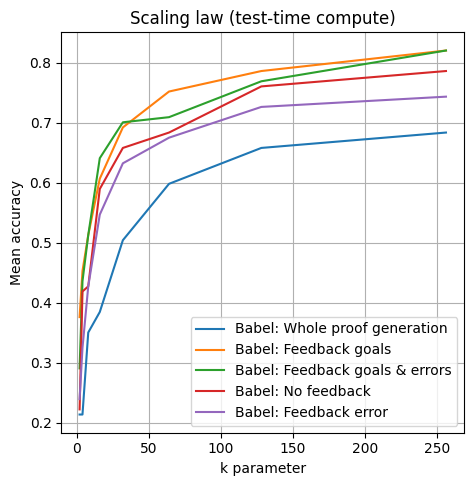
\includegraphics[width=0.4\textwidth]{scaling_feedback}
		\caption{Lean $\to$ Rocq scaling (pass@$k$) for different feedback modes.}
		\label{fig:scaling-feedback}
	\end{figure}
	
	\begin{figure}[!h]
		\centering
		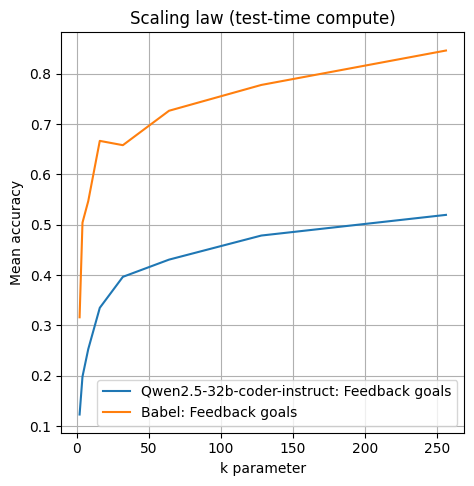
\includegraphics[width=0.4\textwidth]{scaling_compare}
		\caption{Lean $\to$ Rocq scaling (pass@$k$): Babel vs.\ Qwen2.5-Coder-32B-Instruct, with matched sampling budget in the Term $\to$ Script mode.}
		\label{fig:scaling-compare}
	\end{figure}
	
	\section{Conclusion and Future Work}
	
	We introduced proof term translation as a way to translate proofs across assistants and tactic styles. Unlike direct tactic translation, this approach does not need parallel scripts for training. On our benchmarks it brings clear gains for style transfer and remains competitive for cross-assistant translation.
	
	\paragraph{Future work.}
	We see three directions:
	\begin{itemize}
		\item \textbf{Scale.} Train on larger corpora and more domains, since the approach does not require aligned scripts.
		\item \textbf{Multilingual.} Scaling this approach to additional assistants mainly requires: (i) extraction and pretty-printing of proof terms, (ii) an automated verification in the target system. Training data is then easy to obtain from native corpora because we do not require parallel scripts.
		\item \textbf{Source-to-source translation (Lean~$\leftrightarrow$ Rocq).} Use off-the-shelf LLMs for source-to-source translation, and bootstrap proof script translation to check whether the source translation is correct.
	\end{itemize}
	
	% ICML: do not include acknowledgements in the anonymous submission.
	% \section*{Acknowledgements}
	% Omitted for anonymous review.
	
	\section*{Impact Statement}
	This paper studies automated translation of formal proofs between proof assistants and between tactic languages. A primary positive impact is improved interoperability between formal-mathematics ecosystems, which can reduce duplicated effort and accelerate the reuse of verified results. Because all translated scripts are ultimately checked by the target proof assistant, the approach is designed to mitigate the risk of producing incorrect proofs that appear superficially plausible. Remaining risks include engineering misuse (e.g., over-trusting generated scripts before verification, or deploying translation pipelines without adequate checks) and potential shifts in how contributors learn and write proofs. We therefore emphasize verification-first workflows and recommend that tool support surface proof obligations, errors, and provenance of generated artifacts.
	
	\bibliography{babel}
	\bibliographystyle{icml2026}

	\newpage
	\appendix
	\onecolumn
	
	
	\section{Appendix}
	
	
	\subsection{Training Details}
	\label{app:training}
	We fine-tune a pretrained and instruction-tuned \texttt{Qwen2.5-32b-Coder-Instruct}\cite{deepseek2024} for reasoning, following the setup of S1 simple test-time scaling \cite{s12025}. We train for five epochs with a global batch size of 16, which yields 315 gradient steps. We use bfloat16 precision and an AdamW optimizer with $\beta_1=0.9$, $\beta_2=0.95$, and weight decay $1\times 10^{-4}$. The learning rate is $1\times 10^{-5}$, warmed up linearly for the first $5\%$ (16 steps) and then cosine-decayed to zero over the remaining 299 steps. We compute loss only on the reasoning traces and the final solutions, and we choose a sequence length large enough to avoid truncation. On GENCI hardware (8$\times$4 NVIDIA H100), this run completes in about one hour.
	At inference, we sample up to 256 candidates.
	
	
	\subsection{Prompt Babel-translate}
	\label{app:promptbabel}
	For Lean $\to$ Rocq, we instruct the model to translate a Lean proof term and its local context into a Rocq tactic script. We prepend the following instruction:
	\begin{verbatim}
		You are given a proof term:
		
		{term}
		
		Your task is to derive a sequence of tactics that corresponds to this term.
		
		When you work through the problem, write down your reasoning in detail inside
		<think> ... </think> tags. This reasoning should reflect your natural thought
		process as you explore the structure of the term and figure out what tactics
		to apply. You should consider different possible approaches, reflect on why 
		some might or might not work, and gradually converge on a tactic choice.
		
		After each reasoning block, provide the next (group of) tactic(s) enclosed in:
		
		\box{{
				<tactic>
		}}
		
		Some dependencies that could be helpful:
		
		{dependencies}
	\end{verbatim}
	We hard-code the beginning of the first thinking block:
	\begin{verbatim}
		<think> Okay, let's try to transform this proof term into a sequence of coq
		tactics.
		First let's write down the hypotheses, and the initial goal
		(after the "|-" symbol) given by the coq proof assistant:
		{initial_goal}.
	\end{verbatim}
	
	\subsection{Prompt GPT-5 direct translation}
	\label{app:promptgpt}
	For Lean $\to$ Rocq, we instruct the model to translate a Lean proof script into a Rocq proof script. We give the following instruction:
	\begin{verbatim}
		You are a precise translator from Lean 4 proofs to Rocq (Coq).
		
		## INPUT
		<ROCQ_STATEMENT>
		{rocq_statement}
		</ROCQ_STATEMENT>
		
		<LEAN_STATEMENT>
		{lean_statement}
		</LEAN_STATEMENT>
		
		<LEAN_PROOF>
		{lean_proof}
		</LEAN_PROOF>
		
		<DEPENDENCIES>
		{dependencies}
		</DEPENDENCIES>
		
		## RULES
		1) Produce two blocks in this exact order and format:
		a) A thought process.
		b) The final Rocq proof script delimited by the markers below.
		2) Use only lemmas/results listed in <DEPENDENCIES>. Do not rely on
		external lemmas beyond these. Standard Rocq/Coq tactics are allowed.
		3) Do not invent new lemmas.
		4) Do not use "Admitted.". End with "Qed.".
		5) Output must contain only the two blocks below, nothing else.
		
		## OUTPUT FORMAT (STRICT)
		<BEGIN_RATIONALE>
		[Thought process.]
		</END_RATIONALE>
		
		<BEGIN_ROCQ_PROOF>
		[Place only the Rocq/Coq script here. Inside "Proof." ... "Qed.",
		do not rewrite the Rocq statement.]
		</END_ROCQ_PROOF>
		
		Now produce the output for the given input.
	\end{verbatim}
	
	In case of an issue, we prepend the following feedback to the next prompt:
	\begin{verbatim}
		You already tried this proof:
		{proof}
		but it fails with this error:
		{error_message}.
	\end{verbatim}
	
	\subsection{Benchmark example}
	\label{app:benchmark}
	We show one Lean/Rocq pair from the aligned set. The Rocq entry is:
	
	\begin{verbatim}
		Class AbsField := {
			R0   : Type;
			zero : R0;
			one  : R0;
			add  : R0 -> R0 -> R0;
			mul  : R0 -> R0 -> R0;
			opp  : R0 -> R0;
			abs  : R0 -> R0;
			leR  : R0 -> R0 -> Prop;
			ltR  : R0 -> R0 -> Prop;
			
			
			N0       : Type;
			Nle      : N0 -> N0 -> Prop;
			Nmax     : N0 -> N0 -> N0;
			Nle_max_l : forall x y, Nle x (Nmax x y);
			Nle_max_r : forall x y, Nle y (Nmax x y);
			
			add_comm  : forall x y, add x y = add y x;
			add_assoc : forall x y z, add (add x y) z = add x (add y z);
			add_zero  : forall x, add x zero = x;
			add_opp   : forall x, add x (opp x) = zero;
			mul_comm  : forall x y, mul x y = mul y x;
			mul_assoc : forall x y z, mul (mul x y) z = mul x (mul y z);
			mul_one   : forall x, mul x one = x;
			
			le_refl   : forall x, leR x x;
			le_trans  : forall x y z, leR x y -> leR y z -> leR x z;
			add_le_add : forall a b c d, leR a b -> leR c d -> leR (add a c)\\
			(add b d);
			
			abs_nonneg : forall x, leR zero (abs x);
			abs_triangle : forall x y, leR (abs (add x y)) (add (abs x) (abs y));
			abs_opp : forall x, abs (opp x) = abs x;
			abs_sub_symm : forall x y, abs (add x (opp y)) = abs (add y (opp x));
			sub_decomp : forall x y z, add x (opp z) = add (add x (opp y)) \\
			(add y (opp z));
			sub_eq_zero : forall x y, add x (opp y) = zero -> x = y;
			
			
			eq_of_forall_eps2 : forall x, (forall eps, ltR zero eps -> leR \\
			(abs x) (add eps eps)) -> x = zero
		}.
		
		Section Limits.
		Context {A : AbsField}.
		
		Definition sub (x y : R0) : R0 := add x (opp y).
		
		Definition limit (u : N0 -> R0) (l : R0) : Prop :=
		forall eps, ltR zero eps -> exists N, forall n, Nle N n -> leR\\
		(abs (sub (u n) l)) eps.
		
		Lemma abs_sub_triangle (x y z : R0) :
		leR (abs (sub x z)) (add (abs (sub x y)) (abs (sub y z))).
		Proof.
		unfold sub.
		rewrite (sub_decomp x y z).
		apply abs_triangle.
		Qed.
		
		Theorem limit_unique (u : N0 -> R0) (l m : R0) :
		limit u l -> limit u m -> l = m.
		Proof.
		intros Hl Hm.
		assert (Hbound: forall eps, ltR zero eps -> leR (abs (sub l m))\\
		(add eps eps)).
		{ intros eps Heps.
			destruct (Hl eps Heps) as [N1 HN1].
			destruct (Hm eps Heps) as [N2 HN2].
			set (N := Nmax N1 N2).
			assert (H1u: leR (abs (sub (u N) l)) eps).
			{ apply HN1. apply Nle_max_l. }
			assert (H1: leR (abs (sub l (u N))) eps).
			{ unfold sub in H1u. rewrite abs_sub_symm in H1u. fold sub\\
				in H1u. exact H1u. }
			assert (H2: leR (abs (sub (u N) m)) eps).
			{ apply HN2. apply Nle_max_r. }
			assert (Htri: leR (abs (sub l m)) (add (abs (sub l (u N)))\\
			(abs (sub (u N) m)))) by apply abs_sub_triangle.
			eapply le_trans; [exact Htri|].
			apply add_le_add; [exact H1|exact H2].
		}
		assert (Hz: sub l m = zero).
		{ apply eq_of_forall_eps2. exact Hbound. }
		unfold sub in Hz.
		now apply sub_eq_zero in Hz.
		Qed.
		
		End Limits.
	\end{verbatim}
	
	The Lean counterpart is:
	
	\begin{verbatim}
		class AbsField (R : Type) where
		zero  : R
		one   : R
		add   : R → R → R
		mul   : R → R → R
		opp   : R → R
		abs   : R → R
		leR    : R → R → Prop
		ltR    : R → R → Prop
		
		
		NatAlt     : Type
		NatAltle   : NatAlt → NatAlt → Prop
		NatAltMax  : NatAlt → NatAlt → NatAlt
		le_max_left  : forall x y, NatAltle x (NatAltMax x y)
		le_max_right : forall x y, NatAltle y (NatAltMax x y)
		
		add_comm  : forall x y, add x y = add y x
		add_assoc : forall x y z, add (add x y) z = add x (add y z)
		add_zero  : forall x, add x zero = x
		add_opp   : forall x, add x (opp x) = zero
		opp_add   : forall x y, opp (add x y) = add (opp x) (opp y)
		mul_comm  : forall x y, mul x y = mul y x
		mul_assoc : forall x y z, mul (mul x y) z = mul x (mul y z)
		mul_one   : forall x, mul x one = x
		
		le_refl   : forall x, leR x x
		le_trans  : forall x y z, leR x y → leR y z → leR x z
		add_le_add : forall a b c d, leR a b → leR c d → leR (add a c) \\
		(add b d)
		
		abs_nonneg : forall x, leR zero (abs x)
		abs_triangle : forall x y, leR (abs (add x y)) (add (abs x) (abs y))
		abs_opp : forall x, abs (opp x) = abs x
		abs_sub_symm : forall x y, abs (add x (opp y)) = abs (add y (opp x))
		
		
		sub_decomp : forall x y z, add x (opp z) = add (add x (opp y)) \\
		(add y (opp z))
		sub_eq_zero : forall x y, add x (opp y) = zero → x = y
		
		eq_of_forall_eps2 : forall x, (forall eps, ltR zero eps → leR (abs x) \\
		(add eps eps)) → x = zero
		
		namespace Limits
		
		variable {R : Type} [AR : AbsField R]
		
		def sub (x y : R) : R := AbsField.add x (AbsField.opp y)
		
		def limit (u : (AbsField.NatAlt (R := R)) → R) (l : R) : Prop :=
		forall eps : R, AbsField.ltR AbsField.zero eps →
		exists N : AbsField.NatAlt (R := R),
		forall n : AbsField.NatAlt (R := R),
		AbsField.NatAltle (R := R) N n →
		AbsField.leR (AbsField.abs (sub (u n) l)) eps
		
		theorem abs_sub_triangle (x y z : R) :
		AbsField.leR (AbsField.abs (sub x z)) (AbsField.add (AbsField.abs \\
		(sub x y)) (AbsField.abs (sub y z))) := by
		
		have : sub x z = AbsField.add (sub x y) (sub y z) := sub_decomp x y z
		simpa [this] using AbsField.abs_triangle (sub x y) (sub y z)
		
		theorem limit_unique (u : (AbsField.NatAlt (R := R)) → R) (l m : R) :
		limit u l → limit u m → l = m :=
		by
		intro Hl Hm
		
		have Hbound' : forall eps, AR.ltR AR.zero eps → AR.leR (AR.abs (sub l m)) \\
		(AR.add eps eps) := by
		intro eps Heps
		rcases Hl eps Heps with ⟨N1, HN1⟩
		rcases Hm eps Heps with ⟨N2, HN2⟩
		let N := AbsField.NatAltMax (R := R) N1 N2
		have H1 : AbsField.leR (AbsField.abs (sub (u N) l)) eps := by
		apply HN1
		exact AbsField.le_max_left (R := R) _ _
		have H2 : AbsField.leR (AbsField.abs (sub (u N) m)) eps := by
		apply HN2
		exact AbsField.le_max_right (R := R) _ _
		
		have Htri : AbsField.leR (AbsField.abs (sub l m)) (AbsField.add \\
		(AbsField.abs (sub l (u N))) (AbsField.abs (sub (u N) m))) := by
		simpa using abs_sub_triangle l (u N) m
		
		
		have H1' : AbsField.leR (AbsField.abs (sub l (u N))) eps := by
		
		simpa [sub, AbsField.abs_sub_symm (u N) l] using H1
		exact AbsField.le_trans _ _ _ Htri (AbsField.add_le_add _ _ _ _ H1' H2)
		
		have Hz : sub l m = AbsField.zero := AbsField.eq_of_forall_eps2 (sub l m) Hbound'
		
		exact AbsField.sub_eq_zero l m (by simpa [sub] using Hz)
		end Limits
	\end{verbatim}
	
	
	\subsection{Translation to SSReflect}
	\label{app:ssreflect}
	
	We illustrate the Rocq~$\to$~SSReflect translation on a lemma extracted from CoRN. Babel takes as input the proof term and produces a short SSReflect script that closes the goal under the same context.
	
	\paragraph{Lemma (CoRN).}
	\begin{verbatim}
		Lemma CR_nonZero_as_Cauchy_IR_nonZero_1 :
		forall (x:CR), (CRapartT x 0)%CR ->
		Dom (f_rcpcl' _) (CRasCauchy_IR x).
	\end{verbatim}
	
	\paragraph{Proof term.}
	\begin{verbatim}
		CR_nonZero_as_Cauchy_IR_nonZero_1 =
		fun (x : CR) (x_ : (x >< ' 0%Q)%CR) =>
		ap_wdr_unfolded Cauchy_IR (CRasCauchy_IR x) (CRasCauchy_IR (' 0%Q)%CR) [0]
		(CR_ap_as_Cauchy_IR_ap_1 x (' 0%Q)%CR x_)
		(CR_inject_Q_as_Cauchy_IR_inject_Q 0)
		: forall x : CR,
		(x >< ' 0%Q)%CR ->
		Dom (f_rcpcl' Cauchy_IR) (CRasCauchy_IR x)
		
		Arguments CR_nonZero_as_Cauchy_IR_nonZero_1 x _
	\end{verbatim}
	
	\paragraph{Original Rocq script.}
	\begin{verbatim}
		intros x x_.
		change ((CRasCauchy_IR x)[#][0]).
		stepr (CRasCauchy_IR 0%CR).
		apply CR_ap_as_Cauchy_IR_ap_1.
		assumption.
		eapply CR_inject_Q_as_Cauchy_IR_inject_Q.
		Defined.
	\end{verbatim}
	
	\paragraph{Babel (SSReflect) script from the term.}
	\begin{verbatim}
		move=> x_; rewrite /CRapartT; apply: CR_ap_as_Cauchy_IR_ap_1 => /=.
	\end{verbatim}
	
	\subsection{Translation from Lean to Rocq}
	\label{app:leanrocq}
	
	We illustrate the Lean~$\to$~Rocq translation on a lemma whose Lean proof uses the \texttt{simp} tactic. Babel takes as input the proof term and the goal (it does not see the Lean proof), and reconstructs the explicit calls to lemmas such as \texttt{map\_smul} and \texttt{smul\_zeroV} 
	that \texttt{simp} applies implicitly.
	
	\paragraph{Lemma (Lean).}
	\begin{verbatim}
		theorem ker_smul {L : LMap (R:=R) V W} {a : R} {x : V} :
		ker L x → ker L (VSpace.smul (R:=R) a x) :=
		by
		intro hx
		unfold ker at *
		simp [hx]
	\end{verbatim}
	
	\paragraph{Proof term.}
	\begin{verbatim}
		ker_smul =
		fun (VS2 : VSpace) (L : Lin) (a : R0) (x : V0) (hx : ker L x) =>
		eq_ind_r (fun v : V0 => v = zeroV)
		(eq_ind_r (fun v : V0 => (a •V v) = zeroV)
		(eq_ind_r (fun v : V0 => v = zeroV) eq_refl (smul_zeroV a)) hx)
		(map_smul L a x)
		: forall {VS2 : VSpace} (L : Lin) (a : R0) (x : V0),
		ker L x -> ker L (a •V x)
	\end{verbatim}
	
	\paragraph{Original Lean script.}
	\begin{verbatim}
		intro hx
		unfold ker at *
		simp [hx]
	\end{verbatim}
	
	
	\paragraph{Babel (Rocq) reconstruction.}
	
	\noindent\textcolor{red}{The beginning of the first reasoning block (initial hypotheses and goal) is hardcoded by us to provide context; it is \emph{not} generated by the model.}
	
	\begin{verbatim}
		Okay, let's try to transform this proof term into a sequence of Coq tactics.
		First, let's write down the hypotheses and the initial goal (after the "|-") 
		given by the Coq proof assistant:
		
		F  : Field
		VS1, VS2  : VSpace
		L  : Lin
		a  : R0
		x  : V0
		|- ker L x -> ker L (a •V x)
	\end{verbatim}
	
	\noindent\rule{6cm}{0.4pt}
	
	\begin{verbatim}
		The proof term starts with fun {R} ... {x} hx => .... This is a lambda
		abstraction that binds the variable hx. In a Coq proof, this corresponds
		to introducing an assumption. The type of this assumption is the premise
		of the implication in the goal, which is ker L x. So, the first logical
		step is to introduce this assumption into our proof context. The tactic
		for this is intros. The lambda term gives it the name hx, so I'll use
		that. This will change our goal to the conclusion of the implication,
		which is ker L (a •V x). </think>
		\box{intros hx.}
		
		<think> Now, my proof state is:
		F, VS1, VS2, L, a, x : ...
		hx : ker L x
		|- ker L (a •V x)
		
		The goal is ker L (a •V x). This is a definition. To make progress, I
		need to understand what I'm trying to prove. ker is the kernel of a
		linear map, which means it's the set of vectors that the map sends to zero.
		So, ker L (a •V x) should mean L (a •V x) = 0. To make the proof term
		easier to work with, I should unfold this definition. The tactic for
		unfolding definitions in the goal is unfold. Let's apply that to ker in the
		goal. </think>
		\box{unfold ker in |- *.}
		
		<think> The goal has now unfolded to L (a •V x) = Lin.VSpace.zeroV R. The
		lambda term contains L.map_smul a x. This looks like a lemma about linear
		maps and scalar multiplication. It probably states that L (a •V x) =
		a •V (L x). This seems like a very useful fact, as it lets me distribute the
		linear map L over the scalar multiplication •V. My current goal's left-hand
		side is L (a •V x), which is the perfect form to apply this lemma. The tactic
		rewrite is used to apply an equality to the goal. Since map_smul is a lemma
		of the form LHS = RHS, rewrite map_smul will replace LHS with RHS. I expect
		this to change my goal to a •V (L x) = Lin.VSpace.zeroV R. This looks like a
		promising simplification. </think>
		\box{rewrite map_smul.}
		
		<think> My goal is now a •V (L x) = Lin.VSpace.zeroV R. Let's look at my
		hypotheses. I have hx : ker L x. This is still using the ker definition.
		It would be helpful to have this hypothesis in its unfolded form as well,
		L x = Lin.VSpace.zeroV R. This will make it easier to use hx to rewrite parts
		of my goal. I'll use the unfold tactic again, this time on the hypothesis hx.
		</think>
		\box{unfold ker in hx.}
		
		<think> Now my context contains hx : L x = Lin.VSpace.zeroV R, and my goal is
		a •V (L x) = Lin.VSpace.zeroV R. This is great. The term L x in my goal appears
		exactly as the left-hand side of the equality in my hypothesis hx. This is a
		perfect opportunity to use the rewrite tactic. By doing rewrite hx, I can
		replace L x in the goal with Lin.VSpace.zeroV R. I expect this to transform
		my goal into a •V (Lin.VSpace.zeroV R) = Lin.VSpace.zeroV R. </think>
		\box{rewrite hx.}
		
		<think> The goal is now a •V (Lin.VSpace.zeroV R) = Lin.VSpace.zeroV R. Looking
		at the lambda term, I see a reference to Lin.VSpace.smul_zero a. This must be
		the lemma for a •V 0 = 0. My goal's left-hand side, a •V (Lin.VSpace.zeroV R),
		is precisely the form required by this lemma. Once again, rewrite is the tactic
		to use. Applying rewrite smul_zeroV should simplify the left-hand side of my
		goal to Lin.VSpace.zeroV R, making the
		goal Lin.VSpace.zeroV R = Lin.VSpace.zeroV R. </think>
		\box{rewrite smul_zeroV.}
		
		<think> After the last rewrite, my goal is Lin.VSpace.zeroV R = Lin.VSpace.zeroV R.
		This is an equality of a term with itself. This is a trivially true statement. There
		are several tactics to solve such a goal. reflexivity is the most direct one, as it
		is designed specifically for proving t = t. The lambda term structure Eq.trans ...
		(eq_self ...) confirms that the proof concludes by showing both sides are the same
		thing. Therefore, reflexivity is the final step to close the proof. </think>
		\box{reflexivity.}
	\end{verbatim}
	
	\end{document}